\subsection{Radiation Cloud Modelling}\label{sec:radiation}
\noindent The radiation cloud is assumed to be monitored using a number of sensors on the ground (within the disaster space) that collect readings of the radiation cloud intensity and wind velocity every minute of the game. These sensors can be at fixed locations or held by mobile agents.  The radiation cloud diffusion process is modelled in a standard way by a nonlinear Markov field stochastic differential equation,  
\begin{eqnarray*}
\frac{D \text{Rad}({\bf z}, \tau)}{D \tau}=\kappa \triangledown^2 \text{Rad}({\bf z},\tau)-\text{Rad}({\bf z},\tau)\triangledown \cdot {\bf w}({\bf z},\tau)+\sigma({\bf z},\tau)
\end{eqnarray*}
where $D$ is the material derivative, $\text{Rad}({\bf z},\tau)$ is the radiation cloud intensity at location ${\bf z}$ at time $\tau$, $\kappa$ is a fixed diffusion coefficient and $\sigma$ is the radiation source(s) emission rate. The diffusion equation is solved on a regular grid defined across the environment with grid coordinates $G$ (as defined in Section \ref{sec:model}).  Furthermore, the grid is solved at discrete time instances $\tau$.  The cloud is driven by wind forces which vary both spatially and temporally.  These forces induce anisotropy into the cloud diffusion process which is proportional to the wind velocity, ${\bf w}({\bf z},\tau)$.  The wind velocity is drawn from two independent Gaussian processes (GP), one GP for each Cartesian coordinate axis, $w_i({\bf z},\tau)$, of ${\bf w}({\bf z},\tau)$.  The GP captures both the spatial distribution of the wind velocity and the dynamic process resulting from shifting wind patterns such as short term gusts and longer term variations. 

% In our simulation, each spatial wind velocity component is modelled by a squared-exponential GP covariance function, $K$, with fixed input and output scales (although any covariance function can be substituted). Furthermore, as wind conditions may change over time we introduce a temporal correlation coefficient, $\rho$, to the covariance function.  Thus, for a single component, $w_i$, of ${\bf w}$, defined over grid $G$ at times $\tau$ and $\tau^\prime$, the wind process covariance function is, $\text{Cov}(w_i(G,\tau),w_i(G,\tau^\prime))=\rho(\tau,\tau^\prime) K(G,G)$.  We note that, when $\rho=1$ the wind velocities are time invariant (although spatially variant).  Values of $\rho<1$ model wind conditions that change over time.

Using the above model, we are able to create  a radiation cloud moving over the disaster space, thus posing a real challenge both for the HQ (agent and commander) and the responders on the ground, as predictions they can make of where the cloud will move to will be prone to uncertainty both to the simulated wind speed and direction. 


%(\textbf{Steve: in the platform we take the `real' values from the diffusion process i believe. Does the above capture this? We will say that we will add the features you mention below to a future version of the platform where we aim to do both situational awareness and rescue. Add a sentence above to conclude where we took the values from and the process takes into account the  location of radiation source. Also, your notation clashes with the notations in the scenario and Feng's algorithm - please try to align.}
%The cloud intensity and wind velocity are measured by {\it monitor agents} equipped with geiger-counters and anemometers.  These agents are directed to take measurements with greatest information gain in the radiation cloud intensity.  The measurements are folded into the EKF and this refines estimates of the radiation cloud across the grid.  Figure~\ref{radiation_screen_shots} shows example cloud simulations for slow varying (i.e. $\rho=0.99$) and gusty (i.e. $\rho=0.90$) wind conditions.  Figure~\ref{radiation_screen_shots}(a) shows slow varying wind conditions in which case the radiation cloud can be interpolated accurately using sparse sensor measurements and the LFM model.  Alternatively, during gusty conditions the radiation cloud model is more uncertain far from the locations where recent measurements have been taken, as shown in Figure~\ref{radiation_screen_shots}(b).
%
%\begin{figure}[ht] \begin{center}
%    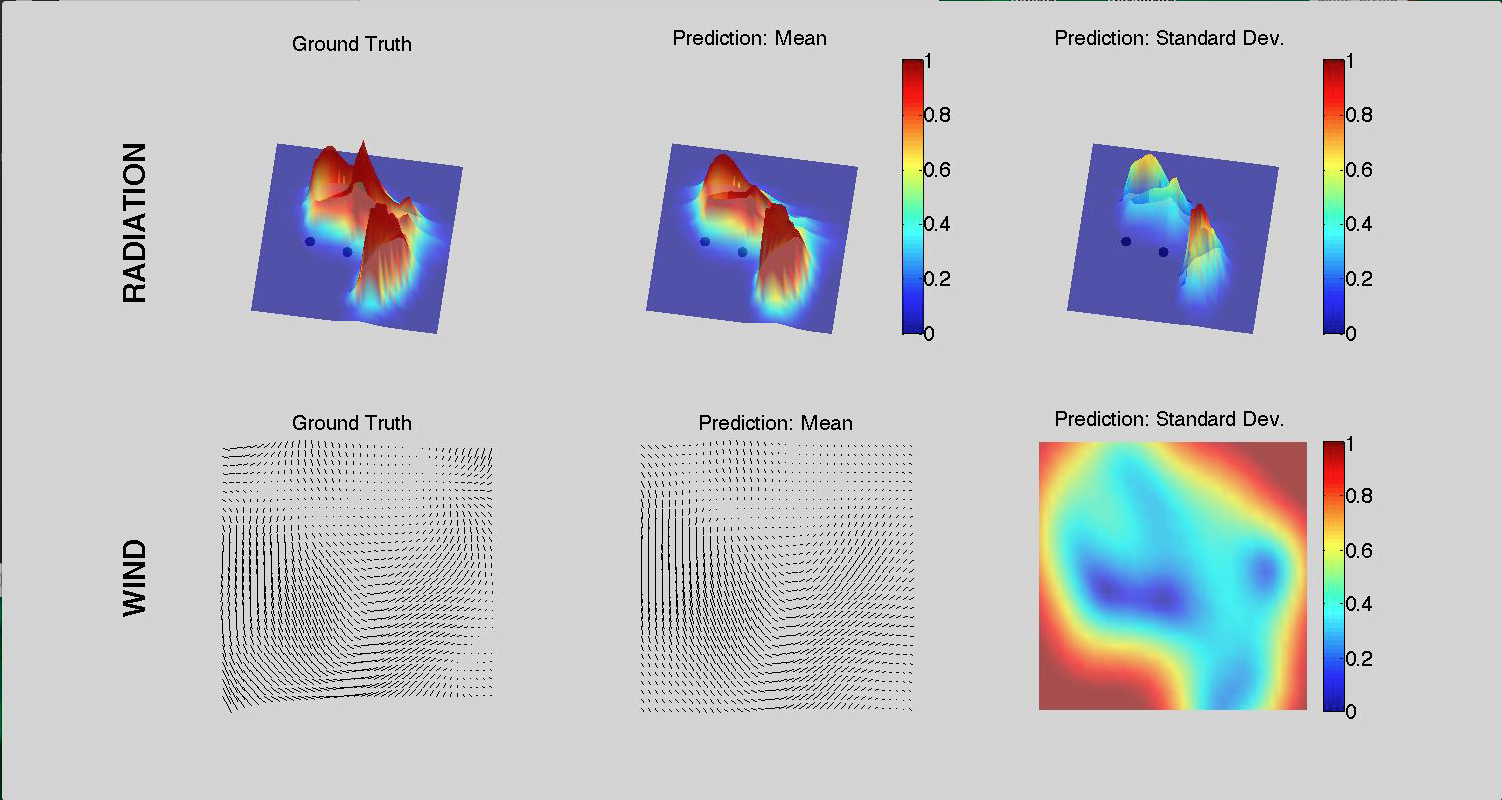
\includegraphics[width=0.45\textwidth]{figures/radiation_ss_calm.png}\\
%    (a) Slowly varying wind conditions\\ \ \\
%    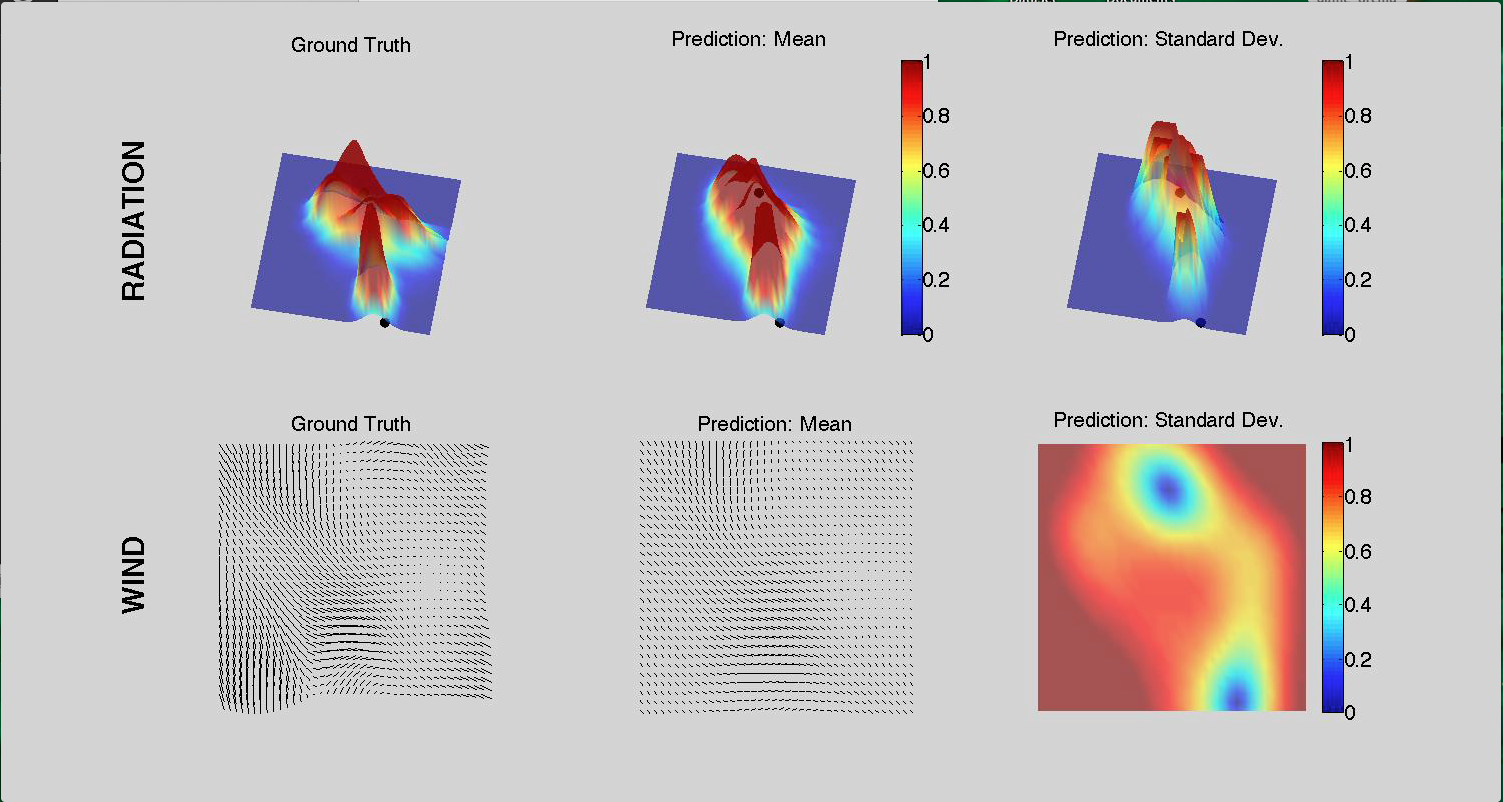
\includegraphics[width=0.45\textwidth]{figures/radiation_ss_gust.png}\\
%    (b) Gusty wind conditions 
%\caption{\label{radiation_screen_shots} Radiation and wind simulation ground truth and EKF estimates obtained using measurements from monitor agents (black dots).  Left most panes are ground truth radiation and wind conditions, the middle panes are corresponding estimates and right most panes are state uncertainties:  (a) Invariant and (b) gusty wind conditions.}
%\end{center}
%\end{figure}
